\documentclass{beamer}

\mode<presentation>
{
  \usetheme{CambridgeUS}
  \usecolortheme{seagull}
  \setbeamercovered{transparent}
}

\usepackage[english]{babel}
\usepackage[latin1]{inputenc}
\usepackage{times}
\usepackage[T1]{fontenc} 
% Or whatever. Note that the encoding and the font should match. If T1
% does not look nice, try deleting the line with the fontenc.
\usepackage{amsmath}

\newcommand{\linespace}{\vskip 0.25cm}

\definecolor{MyForestGreen}{rgb}{0,0.7,0} 
\newcommand{\tableemph}[1]{{#1}}
\newcommand{\tablewin}[1]{\tableemph{#1}}
\newcommand{\tablemid}[1]{\tableemph{#1}}
\newcommand{\tablelose}[1]{\tableemph{#1}}

\definecolor{MyLightGray}{rgb}{0.6,0.6,0.6}
\newcommand{\tabletie}[1]{\color{MyLightGray} {#1}}

% The text in square brackets is the short version of your title and will be used in the
% header/footer depending on your theme.
\title[Concurrent Compaction in JVM GC]{Concurrent Compaction in JVM Garbage Collection}

% Sub-titles are optional - uncomment and edit the next line if you want one.
% \subtitle{Why does sub-tree crossover work?} 

% The text in square brackets is the short version of your name(s) and will be used in the
% header/footer depending on your theme.
\author[Jacob Opdahl]{Jacob P. Opdahl}


% The text in square brackets is the short version of your institution and will be used in the
% header/footer depending on your theme.
\institute[UMM]
{
  University of Minnesota, Morris \\[\baselineskip]
  \emph{opdah023@morris.umn.edu}
}

% The text in square brackets is the short version of the date if you need that.
\date[December 5, 2015] % (optional)
{December 5, 2015}

% Delete this, if you do not want the table of contents to pop up at
% the beginning of each subsection:
%\AtBeginSection[]
%{
%  \begin{frame}<beamer>
%    \frametitle{Outline}
%    \tableofcontents[currentsection, hideothersubsections]
%  \end{frame}
%}

\begin{document}

\begin{frame}
  \titlepage
\end{frame}

% For a 20-25 minute senior seminar talk you probably want something like:
% - Two or three major sections (other than the summary).
% - At *most* three subsections per section.
% - Talk about 30s to 2min per frame. So there should probably be between
%   15 and 30 frames, all told.



\section*{Overview}

\subsection*{Introduction}

\begin{frame}

\frametitle{Automatic Memory Management}

Implicit allocation and deallocation of memory

\linespace
\linespace

Languages: Java, C\#, Python, and more
\begin{itemize}
\item We focus on the Java Virtual Machine and languages it supports
\end{itemize}

\linespace
\linespace

Abstracts details away from the developer

\linespace

\begin{center}

\includegraphics[width=.3\textwidth]{Illustrations/garbage.jpg}
\end{center}

\end{frame}

\begin{frame}

\frametitle{Implicit Deallocation}

Memory is a finite resource

\linespace
\linespace

\emph{garbage}: objects that are no longer reachable

\linespace
\linespace

\emph{garbage collector}: algorithm for detecting and removing garbage
\begin{itemize}
\item Performs garbage collection (GC)
\end{itemize}

\linespace

\begin{center}

\includegraphics[width=.3\textwidth]{Illustrations/garbage.jpg}
\end{center}

\end{frame}

\begin{frame}

\frametitle{Stopping the World}

GC requires processing resources

\linespace
\linespace

When only one processor is used, collectors stop the world

\linespace
\linespace

Problem: applications today are subjected to increasing pauses
\begin{itemize}
\item More memory
\item More strenuous applications
\end{itemize}

\linespace
\linespace

Use parallel processing to solve!

\end{frame}



\subsection*{Outline}

\begin{frame}
  \frametitle{Outline}
  \tableofcontents  
  %\tableofcontents[hidesubsections]
\end{frame}



\section[Background]{Background}

\subsection[GC Basics]{Garbage Collection}

%Kristin liked the heap visualization I did when explaining it (did with my hands at the time).

\subsection[PP Basics]{Parallel Processing}



\subsection[GC with PP]{Garbage Collection with Parallel Processing}



\section[C4]{Continuously Concurrent Compacting Collector (C4)}

\begin{frame}

\frametitle{Continuously Concurrent Compacting Collector (C4)}

C4 is a full garbage collector

\linespace
\linespace

\emph{generational}: performs GC on "young" and "old" generations

\linespace
\linespace

Intended for large server environments

\linespace
\linespace

Commercially available through Azul Systems

\linespace
\linespace
\linespace

\begin{center}
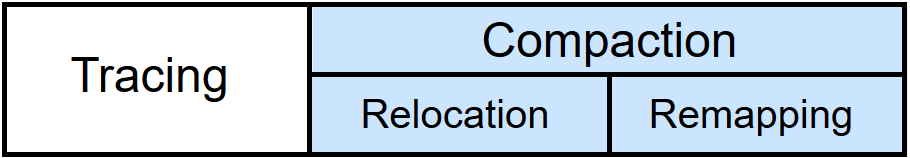
\includegraphics[width=.85\textwidth]{Illustrations/gc_cycle_locator_compaction.png}
\end{center}

\end{frame}



\subsection*{Explanation}

\begin{frame}

\frametitle{The Loaded Value Barrier (LVB)}

Read barrier protects from-space from application threads

\linespace
\linespace

Rule: application can only use moved objects

\linespace
\linespace

If a thread breaks this, the barrier will correct the situation:
\begin{itemize}
\item This facilitates concurrent relocation and remapping
\end{itemize}

\end{frame}

\begin{frame}

\frametitle{Concurrent Relocation}

\only<1>{

GC threads simply relocate objects

\linespace
\linespace

All references point to from-space!
\begin{itemize}
\item Application threads certain to trigger LVB
\end{itemize}

\linespace
\linespace

\begin{center}
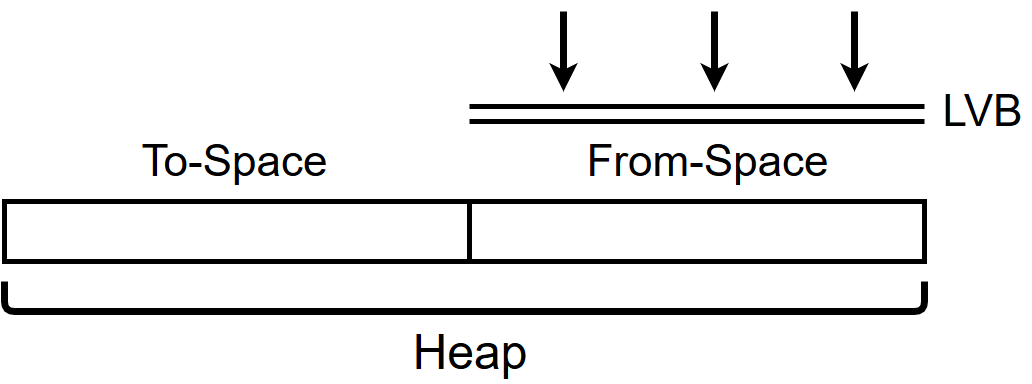
\includegraphics[width=.9\textwidth]{Illustrations/c4_lvb_relocation.png}
\end{center}

}

\only<2>{

How application threads cope:
\begin{itemize}
\item If the object was moved, find it
\item If the object is being moved, wait
\item If the object is unmoved, move it
\end{itemize}

\linespace
\linespace

In all cases, correct the source reference after

}

\end{frame}

\begin{frame}

\frametitle{Concurrent Remapping}

\only<1>{
\emph{lazy remapping}: application threads update references through LVB
\begin{itemize}
\item "If the object was moved, find it"
\item Correct the source reference after
\end{itemize}

\linespace
\linespace

To update all references, need to traverse all reachable ones

\linespace
\linespace

Combine remapping with next tracing phase
}

\only<2>{
\begin{center}
Remapping combined with tracing
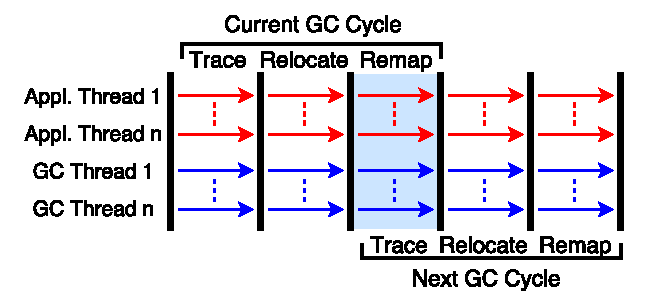
\includegraphics[width=.9\textwidth]{Illustrations/c4Mapping_rough_figure_4.pdf}
\end{center}
}

\end{frame}



\subsection*{Test Results}

\begin{frame}

\frametitle{Testing Environment}

Tested against three garbage collectors:
\begin{itemize}
\item Non-generational version of C4
\item Two algorithms with non-concurrent compaction
\end{itemize}

\linespace
\linespace

Custom benchmarks used to test latency
\begin{itemize}
\item Improvement from a generational collector
\item Improvement from concurrent compaction
\end{itemize}

\end{frame}

\begin{frame}

\frametitle{Results}

%Show the figures from the paper here and start talking about them
\only<1>{
\begin{center}
Application Worst Case Response Times
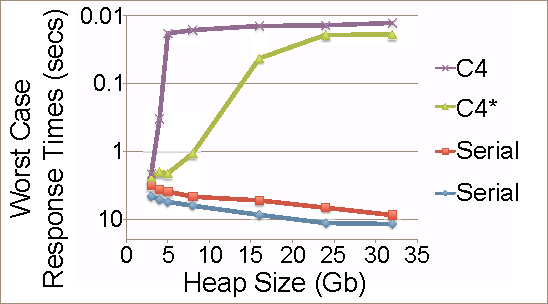
\includegraphics[width=.80\textwidth]{Illustrations/c4_results.pdf}
\end{center}
}

\only<2>{
\begin{columns}
\begin{column}{0.5\textwidth}

\color[RGB]{176,30,186}C4 \color{black}:
\begin{itemize}
\item Has shortest response times
\item Maintains them for largest range of heap sizes
\item Least impact on application
\end{itemize}

\linespace
\linespace

Priority given to GC process

\linespace
\linespace

Still has best application responsiveness

\end{column}

\begin{column}{0.5\textwidth}
\begin{center}
Worst Case Times
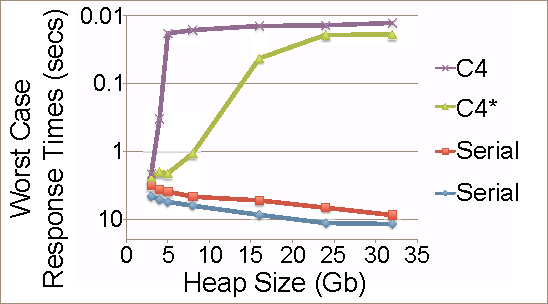
\includegraphics[width=.89\textwidth]{Illustrations/c4_results.pdf}
\end{center}
\end{column}
\end{columns}
}

\end{frame}



\section[Collie]{Collie Collector}

\begin{frame}

\frametitle{Collie Garbage Collector}

Collie is a full garbage collector
\begin{itemize}
\item Uses most techniques from C4
\end{itemize}

\linespace

Also intended for server environments

\linespace

Uses transactional memory for synchronization

\linespace

Major focus on improving latency

\linespace
\linespace
\linespace

\begin{center}
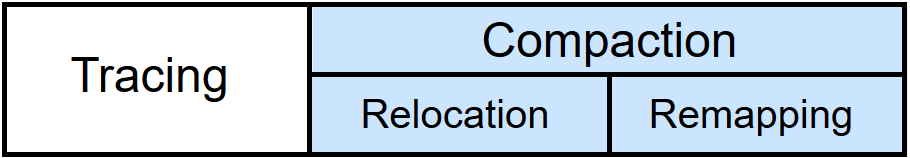
\includegraphics[width=.85\textwidth]{Illustrations/gc_cycle_locator_compaction.png}
\end{center}

\end{frame}



\subsection*{Explanation}

\begin{frame}

\frametitle{Transactions}

%Remember to emphasize the key point is interruptions will cause nothing to happen, or everything to.
\emph{transaction}: series of operations performed in an all-or-none manner

\linespace
\linespace

Example: updating prices in a store for sales \\
\begin{itemize}
\item Update sale price
\item Update store price
\end{itemize}

\linespace
\linespace

Protects data from interrupts

\linespace
\linespace

\emph{transactional memory}: allows code sections to run like transactions
\begin{itemize}
\item Memory used by the code is protected
\end{itemize}

\end{frame}

\begin{frame}

\frametitle{Transplantations}

\emph{transplantation}: Relocating and remapping objects

\linespace
\linespace

\begin{columns}
\begin{column}{0.33\textwidth}

Transaction:
\begin{itemize}
\item Start transaction
\item Check object
\item Relocate object
\item Remap references
\item End Transaction
\end{itemize}

\end{column}
\begin{column}{0.32\textwidth}

$\xrightarrow{\text{Interrupted by application}}$

\end{column}
\begin{column}{0.3\textwidth}

Mark object as non-individually transplantable (NIT)

\end{column}
\end{columns}

\end{frame}

\begin{frame}
%either cut talking about the details or mention that heap is virtual memory earlier.

\frametitle{Leftovers}

\begin{columns}
\begin{column}{0.5\textwidth}
What happens to NIT objects?

\linespace
\linespace

Lie to the compactor:
\begin{itemize}
\item Mirrored-to-space
\item Zero-copy transplantation
\end{itemize}

\linespace
\linespace

\emph{aborting} compactor: no progress guarantees
\end{column}
\begin{column}{0.5\textwidth}

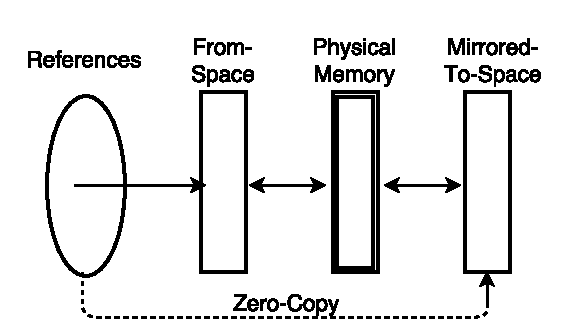
\includegraphics[width=.95\textwidth]{Illustrations/collie_mirrored_rough.pdf}

\end{column}
\end{columns}

\end{frame}



\subsection*{Test Results}

\begin{frame}

\frametitle{Testing Environment}

Tested against the Pauseless Garbage Collector:
\begin{itemize}
\item Ancestor of Collie
\item Largely concurrent with some stop-the-world pauses
\item Also requires supportive hardware
\end{itemize}

\linespace
\linespace

Standard JVM benchmarks used to test latency
\begin{itemize}
\item Improvements from aborting nature and transactions
\end{itemize}

\end{frame}

\begin{frame}

\frametitle{Results}

\only<1>{
\begin{center}
Minimum Mutator Utilization (MMU) Percentages \\for Various Time Windows\\
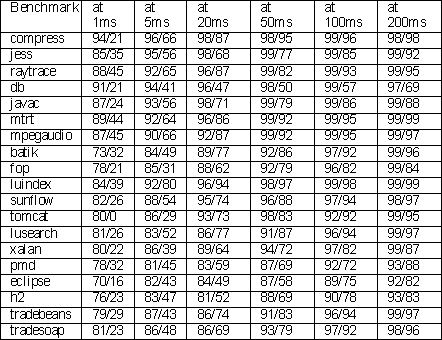
\includegraphics[width=.65\textwidth]{Illustrations/collie_results.pdf}
\end{center}
}

\only<2>{
\begin{center}
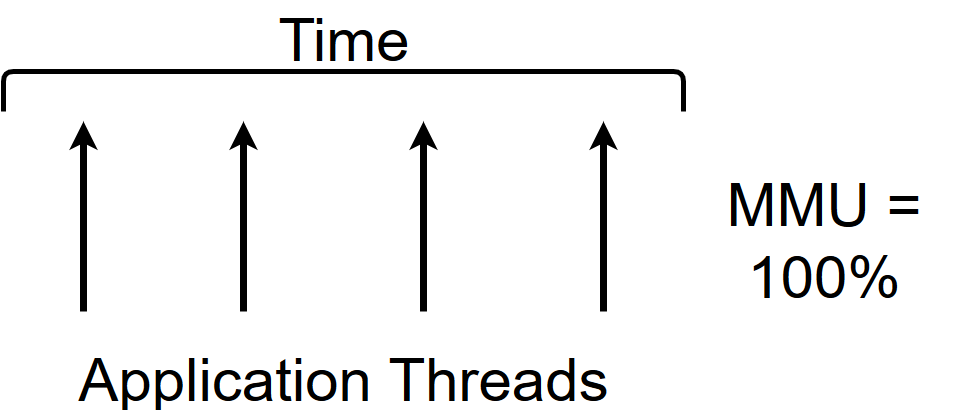
\includegraphics[width=.80\textwidth]{Illustrations/collie_mmu_explanation_1.png}
\end{center}
}

\only<3>{
\begin{center}
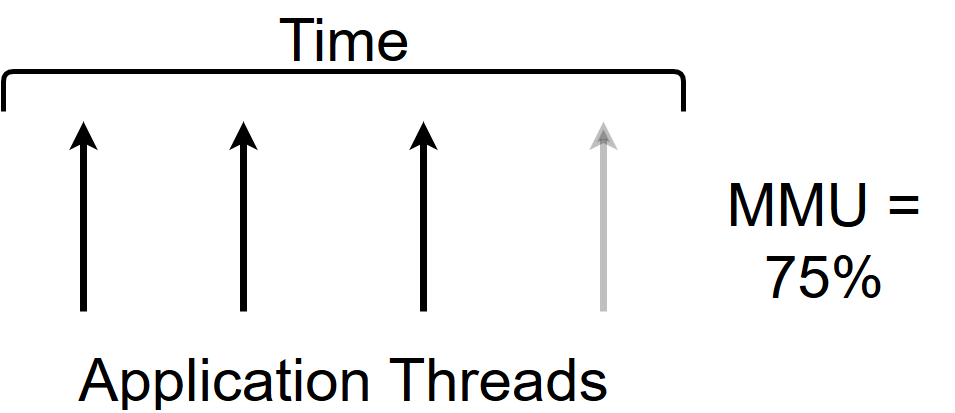
\includegraphics[width=.80\textwidth]{Illustrations/collie_mmu_explanation_2.png}
\end{center}
}

\only<4>{
\begin{columns}
\begin{column}{0.5\textwidth}

\color{red}Collie \color{black}has higher MMU than \color{blue}Pauseless \color{black}across the board
\begin{itemize}
\item Application threads used more
\end{itemize}

\linespace
\linespace

Application threads have priority over GC threads

\linespace
\linespace

Lends itself well to latency but no progress guarantees

\end{column}

\begin{column}{0.5\textwidth}
\begin{center}
MMU Percentages
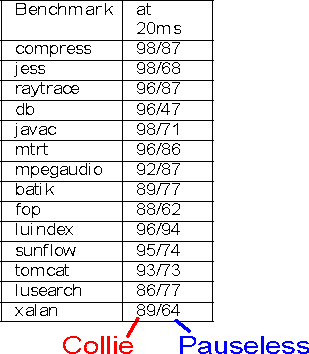
\includegraphics[width=.90\textwidth]{Illustrations/collie_results_2.pdf}
\end{center}
\end{column}
\end{columns}
}

\end{frame}



\section[FPP]{Field Pinning Protocol}

\begin{frame}

\frametitle{Field Pinning Protocol (FPP)}

Solely describes concurrent relocation

\linespace
\linespace

Implements into a host garbage collector
\begin{itemize}
\item Designed for flexibility
\end{itemize}

\linespace
\linespace

Performs relocation without barriers!

\linespace
\linespace
\linespace
\linespace

\begin{center}
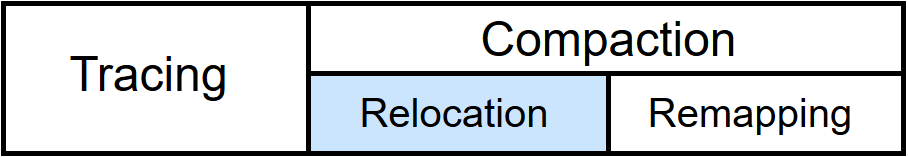
\includegraphics[width=.85\textwidth]{Illustrations/gc_cycle_locator_relocation.png}
\end{center}

\end{frame}



\subsection*{Explanation}

\begin{frame}

\frametitle{Hazard Pointers}

Point to objects an application thread is accessing
\begin{itemize}
\item \emph{Pin} the object
\end{itemize}

\linespace
\linespace

Inform other threads of objects that are in use

\linespace
\linespace

Are maintained by the thread they belong to

\linespace
\linespace

Main goal: safely access objects without worrying about relocation

%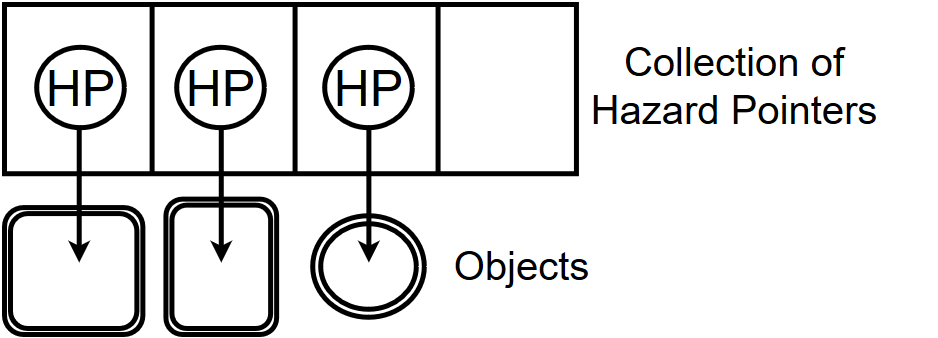
\includegraphics[width=.95\textwidth]{Illustrations/FPP_HP_Illustration.png}


\end{frame}


\begin{frame}

\frametitle{Example}

\begin{columns}
\begin{column}{0.45\textwidth}
	\begin{itemize}
	\item Object = Coffee 
	\item \color{red}{Application Thread = Person w/ Coffee Cup} 
	\only<2->{\item \color{blue}{Relocation Thread = Person}}
	\only<2->{\item \color{black}{* = Responsible}} 
	\only<2->{\item ! = Impeded}
	\end{itemize}
\end{column}
\begin{column}{0.55\textwidth}
	\only<1>{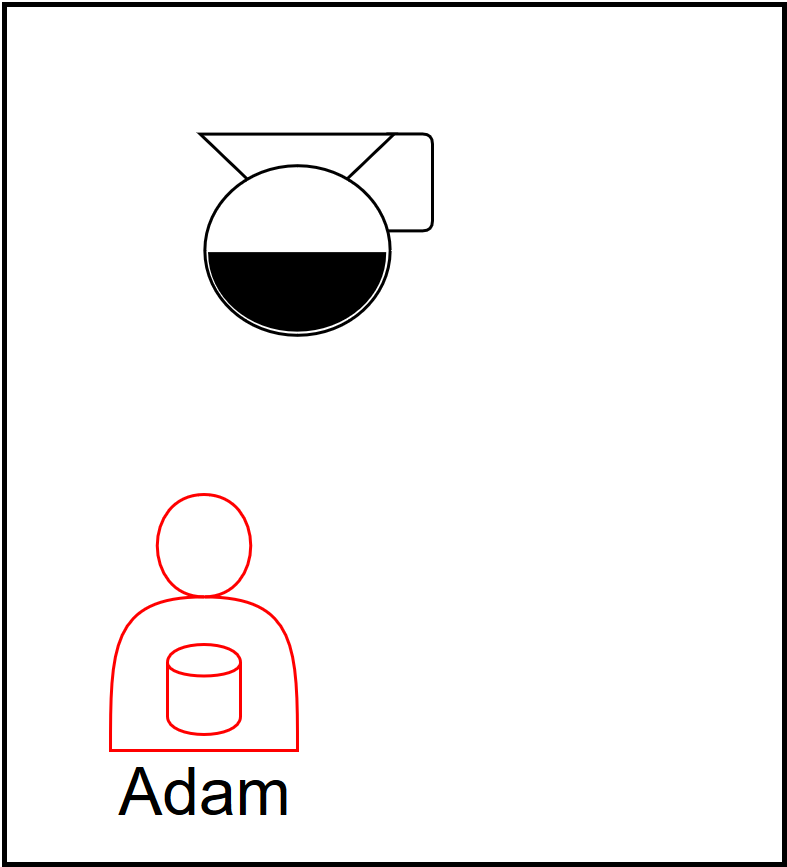
\includegraphics[width=.95\textwidth]{Illustrations/coffeeLineNew1.png}}
	\only<2>{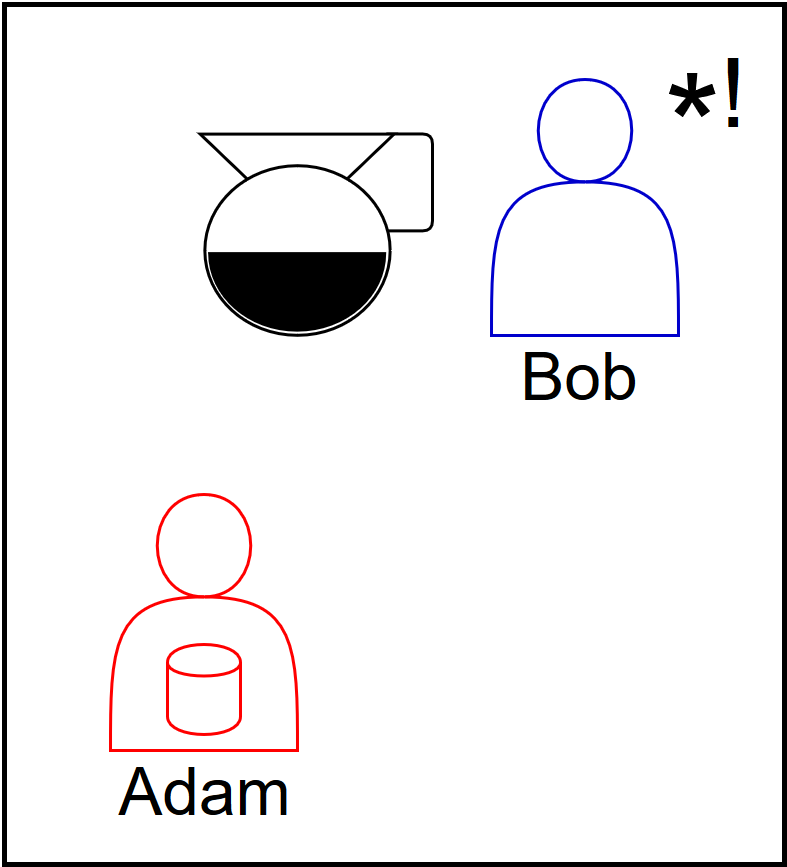
\includegraphics[width=.95\textwidth]{Illustrations/coffeeLineNew2.png}}
	\only<3>{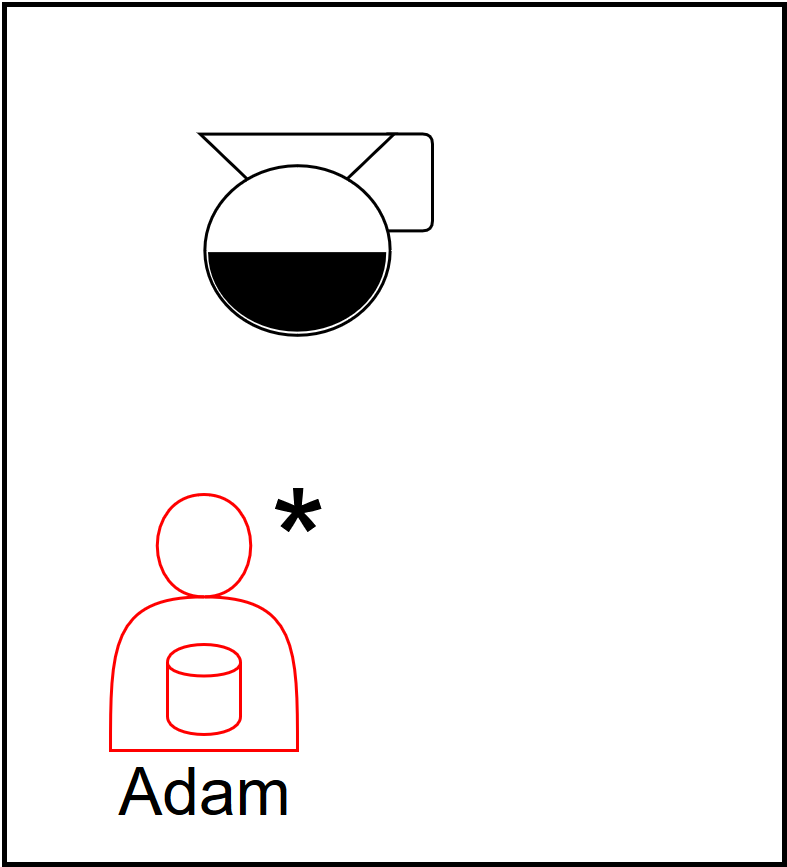
\includegraphics[width=.95\textwidth]{Illustrations/coffeeLineNew3.png}}
	\only<4>{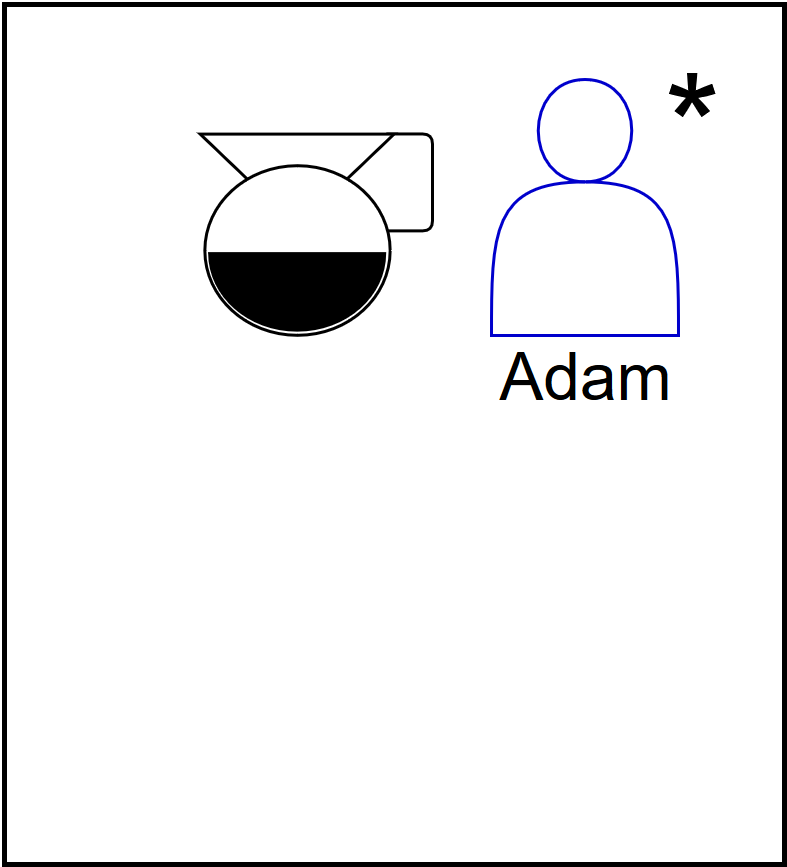
\includegraphics[width=.95\textwidth]{Illustrations/coffeeLineNew4.png}}
	\only<5>{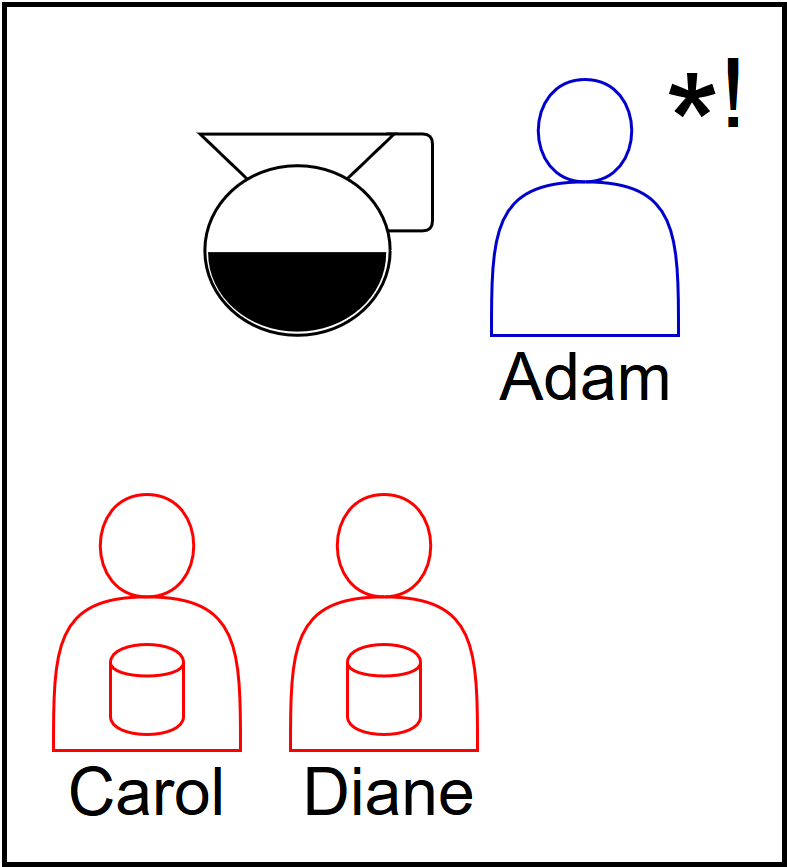
\includegraphics[width=.95\textwidth]{Illustrations/coffeeLineNew5.png}}
\end{column}
\end{columns}

\end{frame}


\begin{frame}

\frametitle{The Blame Game}

%If time allows and feedback demands, could break this into multiple slides to not have so much text
%on one as well as to refer back to the example and characters more.

\emph{blamed} thread: responsible for relocating an object
\begin{itemize}
\item Comes from hazard pointers (coffee cups) impeding copying
\end{itemize}

\linespace
\linespace

When relocation begins:
\begin{itemize}
\item GC threads attempt to relocate objects
\begin{itemize}
\item No blame passed!
\end{itemize}
\item GC threads try again
\begin{itemize}
\item Blame interrupting threads
\end{itemize}
\item Blame passed to interrupting threads until relocation succeeds
\end{itemize}

\end{frame}


\begin{frame}

\frametitle{An Application Thread's Perspective}

Process followed by an \color{red}{application thread}\color{black}{:}
\linespace

\begin{columns}
\begin{column}{0.5\textwidth}
\begin{enumerate}
\item Pin object with a hazard pointer
\item Check if the object has been moved already
\item Use the object without worry
\item Unpin the object when done
\item If blamed, try to relocate the object
\end{enumerate}
\end{column}

\begin{column}{0.5\textwidth}
\begin{enumerate}
\item Get a coffee cup
\item Check that the coffee is still in the room
\item Drink all the coffee you want
\item Discard your coffee cup
\item If blamed, try to move the coffee
\end{enumerate}
\end{column}
\end{columns}

\end{frame}



\subsection*{Test Results}

\begin{frame}

\frametitle{Testing Environment}

Implemented in the Garbage-First (G1) Garbage Collector:
\begin{itemize}
\item Concurrent tracing
\item Compaction requires stop-the-world pauses
\end{itemize}

\linespace
\linespace

Tested against the default G1 collector

\linespace
\linespace

Standard JVM benchmarks used to test latency
\begin{itemize}
\item Improvements from concurrent relocation alone
\item Feasibility of barrier-free relocation
\end{itemize}

\end{frame}

\begin{frame}

\frametitle{Results}

%Show the figures from the paper here and start talking about them
\only<1>{
\begin{center}
Average GC Pauses for Various Benchmarks
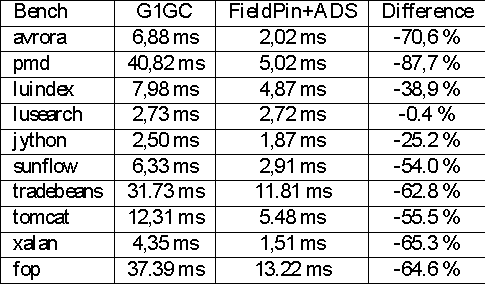
\includegraphics[width=.80\textwidth]{Illustrations/fpp_results.pdf}
\end{center}
}

\only<2>{
\begin{columns}
\begin{column}{0.5\textwidth}

\color{red}G1 with FPP \color{black}on average 50\% shorter pauses than \color{blue}standard G1\color{black}
\begin{itemize}
\item Less impact on application thread performance
\end{itemize}

\linespace
\linespace

Concurrent relocation prioritizes application threads
\begin{itemize}
\item Most latency from host activities
\end{itemize}

\linespace
\linespace

Concurrent relocation without barriers is feasible

\end{column}

\begin{column}{0.5\textwidth}
\begin{center}
Average GC Pauses
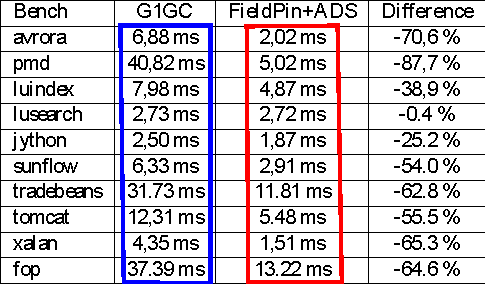
\includegraphics[width=.90\textwidth]{Illustrations/fpp_results_2.pdf}
\end{center}
\end{column}
\end{columns}
}

\end{frame}



\section[Conclusions]{Conclusions}

\begin{frame}
	\frametitle{Thanks for your time!}
	
	\begin{center}
	{\huge Questions?}
	\end{center}	
	
	\linespace
	\linespace	
	
	\begin{center}
	Contact: opdah023@morris.umn.edu
	\end{center}
	
\end{frame}



\section*{References}

\begin{frame} 
	\frametitle{References} 
	
%	\begin{thebibliography}{lskdjf}
%	
%	\bibitem{McPhee:2009:gecco}
%N.~F. McPhee, E.~Crane, S.~Lahr, and R.~Poli.
%\newblock Developmental Plasticity in Linear Genetic Programming.
%\newblock In G\"unther Raidl, \emph{et al}, editors, {\em GECCO '09}, pages 1019--1026, Montr\'eal, Qu\'ebec, Canada, 2009.
%	
%	\bibitem{citeulike:3452411}
%	R.~Poli and N.~McPhee.
%\newblock A linear estimation-of-distribution {GP} system.
%\newblock In M.~O'Neill, \emph{et al}, editors, {\em EuroGP 2008}, volume
%  4971 of {\em LNCS}, pages 206--217, Naples,
%  26-28 Mar. 2008. Springer.
%  
%  	\end{thebibliography}
%	
%	\linespace
%	\begin{center}
%	See the GECCO '09 paper for additional references.
%	\end{center}

\begin{thebibliography}{lskdjf}

\bibitem{Lowe:2015}
E.~\"{O}sterlund and W.~L\"{o}we.
\newblock Concurrent compaction using a field pinning protocol. 
\newblock 2015 ACM SIGPLAN International Symposium on Memory Management (ISMM 2015). ACM, New York, NY, USA, 56-69.

\end{thebibliography}

\end{frame} 



\end{document}


